%%%%%%%%%%%%%%%%%%%%%%%%%%%%%%%%%%%%%%%%%
% University/School Laboratory Report
% LaTeX Template
% Version 3.1 (25/3/14)
%
% This template has been downloaded from:
% http://www.LaTeXTemplates.com
%
% Original author:
% Linux and Unix Users Group at Virginia Tech Wiki 
% (https://vtluug.org/wiki/Example_LaTeX_chem_lab_report)
%
% License:
% CC BY-NC-SA 3.0 (http://creativecommons.org/licenses/by-nc-sa/3.0/)
%
%%%%%%%%%%%%%%%%%%%%%%%%%%%%%%%%%%%%%%%%%

%----------------------------------------------------------------------------
%	PACKAGES AND DOCUMENT CONFIGURATIONS
%----------------------------------------------------------------------------

\documentclass{article}

%\usepackage[version=3]{mhchem} 
	% Package for chemical equation typesetting
%\usepackage{siunitx}
	% Provides the \SI{}{} and \si{} command for typesetting SI units
\usepackage{graphicx} 
	% Required for the inclusion of images
\graphicspath{ {LaTeX_Images/} }
	% Directory where images are imported from
%\usepackage{natbib} 
	% Required to change bibliography style to APA
\usepackage{amsmath} 
	% Required for some math elements 

\setlength\parindent{0pt} 
	% Removes all indentation from paragraphs

%\renewcommand{\labelenumi}{\alph{enumi}.} 
	% Make numbering in the enumerate environment by letter rather than 
	% number (e.g. %section 6)

%\usepackage{times} 
	% Uncomment to use the Times New Roman font

\renewcommand{\vec}[1]{\mathbf{#1}}
%\renewcommand{\textfraction}{0.05}

\usepackage{subfigure}
	% Place figures side by side

%----------------------------------------------------------------------------
%	ABSTRACT
%----------------------------------------------------------------------------

\begin{document}

\begin{abstract}
Throughout the first half of this course on digital systems, we have learned 
to design combination systems. In this project we built a combinational 
circuit of a BCD-to-seven-segment display decoder by going through the process 
of designing digital systems from the high-level specification to the final 
implementation.  We defined the encoding scheme of the input and output, 
created the truth table, used K-maps to methodically find minimal switching 
expressions, transformed AND-OR expressions to two-level NAND expressions, 
and implemented and simulated the gate network on Vivado.
\end{abstract}

%----------------------------------------------------------------------------
%	SWITCHING FUNCTIONS
%----------------------------------------------------------------------------

\section{Switching Functions of the Circuit}
The following are minimal switching expressions in NAND-NAND form and their 
respective schematic representation for the function of the circuit.\\

\begin{equation*}
\begin{split}
a & = [ (x_2 x_0)'  (x_1)'  (x_3)'  (x'_2 x'_0)']' \\
  & = NAND(NAND(x_2, x_0), x'_1, x'_3, NAND(x'_2, x'_0)) \\
\end{split}
\end{equation*}
\begin{figure}[h!]
\centering
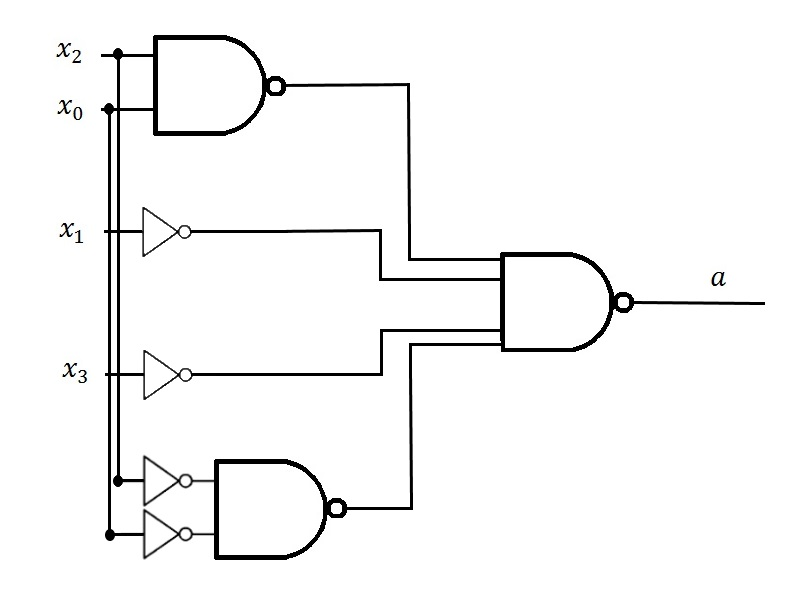
\includegraphics[scale=0.25]{a-NAND-NAND}
\end{figure}

\begin{equation*}
\begin{split}
b & = [ (x_3)' (x_1 x_0)' (x'_1 x'_0)' x_2 ]' \\
  & = NAND(x'_3, NAND(x_1, x_0), NAND(x'_1, x'_0), x_2) \\
\end{split}
\end{equation*}
\clearpage
\begin{figure}[ht]
\centering
\includegraphics[scale=0.25]{b-NAND-NAND}
\end{figure}


\begin{equation*}
\begin{split}
c & = [ (x_3)' x_1 (x_0)' (x_2)' ]' \\ 
  & = NAND(x'_3, x_1, x'_0, x'_2) \\
\end{split}
\end{equation*}
\begin{figure}[h!]
\centering
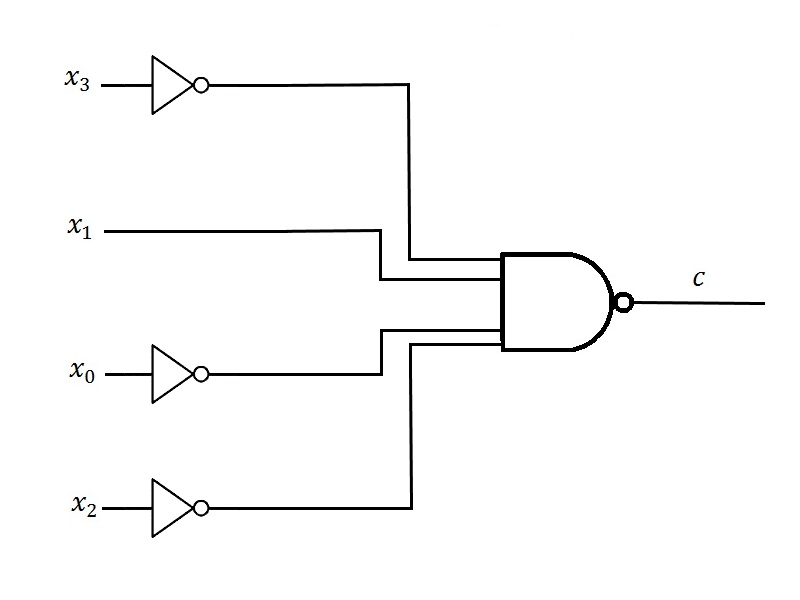
\includegraphics[scale=0.25]{c-NAND-NAND}
\end{figure}


\begin{equation*}
\begin{split}
d & = [ (x_2 x'_1 x_0)' (x'_2 x'_0)' (x_3)' (x_1 x'_0)' (x'_2 x_1)' ]' \\ 
  & = NAND(NAND(x_2, x'_1, x_0), NAND(x'_2, x'_0), x'_3, NAND(x_1, x'_0), 
      NAND(x'_2, x_1)) \\
\end{split}
\end{equation*}
\begin{figure}[h!]
\centering
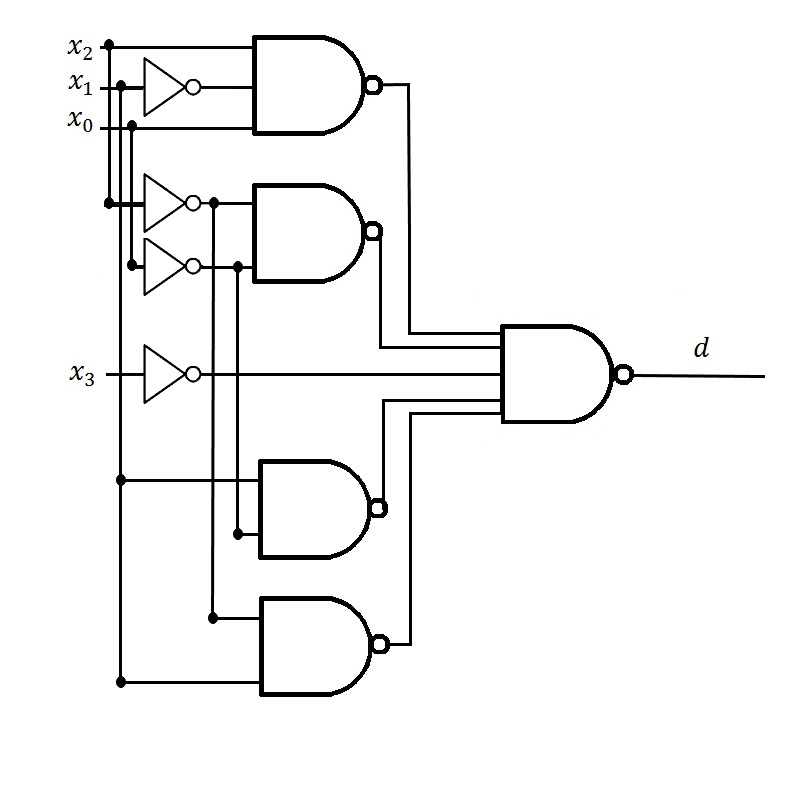
\includegraphics[scale=0.25]{d-NAND-NAND}
\end{figure}

\clearpage


\begin{equation*}
\begin{split}
e & = [ (x'_2 x'_0)' (x_1 x'_0)' ]' \\ 
  & = NAND(NAND(x'_2, x'_0), NAND(x_1, x'_0)) \\
\end{split}
\end{equation*}
\begin{figure}[h!]
\centering
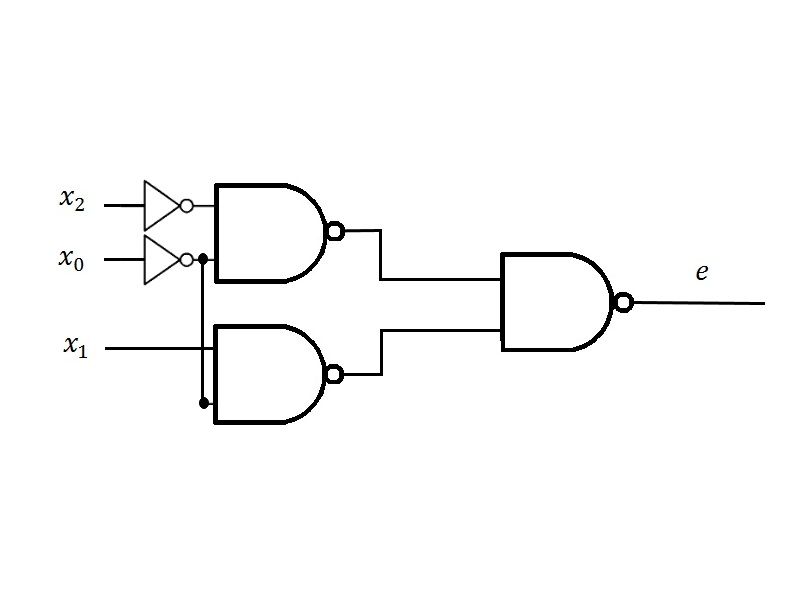
\includegraphics[scale=0.25]{e-NAND-NAND}
\end{figure}


\begin{equation*}
\begin{split}
f & = [ (x_3)' (x_2 x'_0)' (x_2 x'_1)' (x'_1 x'_0)' ]' \\ 
  & = NAND(x'_3, NAND(x_2, x'_0), NAND(x_2, x'_1), NAND(x'_1, x'_0)) \\
\end{split}
\end{equation*}
\begin{figure}[h!]
\centering
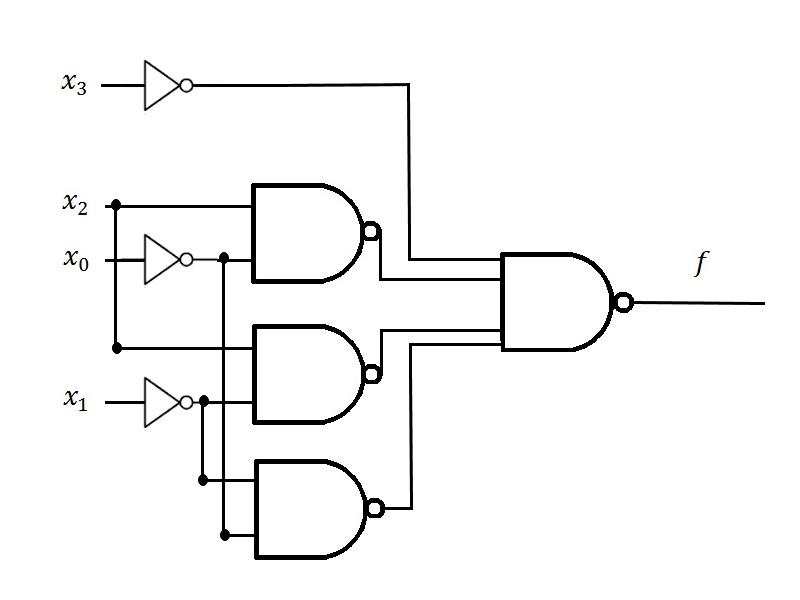
\includegraphics[scale=0.25]{f-NAND-NAND}
\end{figure}

\clearpage


\begin{equation*}
\begin{split}
g & = [ (x_2 x'_1)' (x_3)' (x'_2 x_1)' (x_2 x'_0)' ]' \\ 
  & = NAND(NAND(x_2, x'_1), x'_3, NAND(x'_2, x_1), NAND(x_2, x'_0)) \\
\end{split}
\end{equation*}
\begin{figure}[h!]
\centering
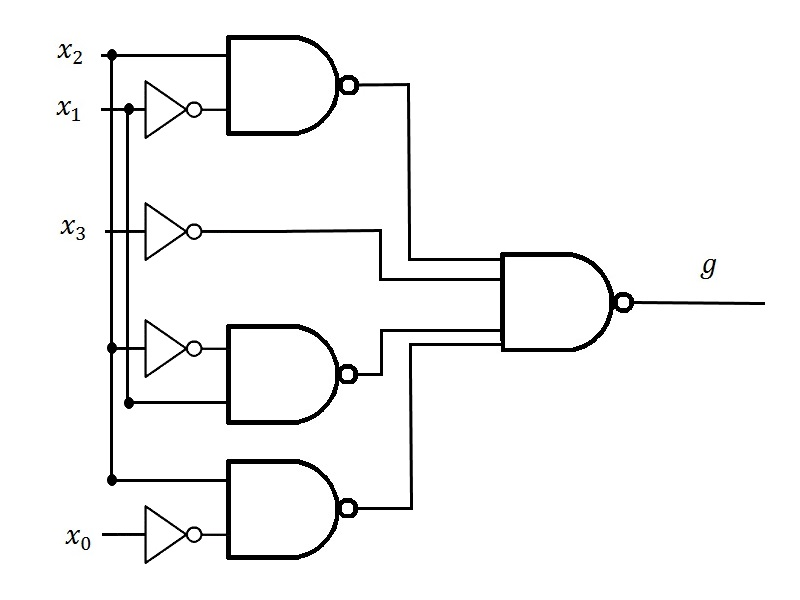
\includegraphics[scale=0.25]{g-NAND-NAND}
\end{figure}

The same expressions can also be found in the Appendix. The Appendix gives a 
step-by-step procedure to get those expressions.
 
%----------------------------------------------------------------------------
%	VERILOG CODE
%----------------------------------------------------------------------------

\section{Verilog Code}
The following is the implementation of our module in code, pasted from a 
Verilog file. Please also refer to \textit{csm51a\_proj2.v} in the zipped 
file.\\

\begin{verbatim}
`timescale 1ns / 1ps
////////////////////////////////////////////////////////////////////////////
// Company: UCLA Henry Samueli School of Engineering and Applied Science
// Engineers: Victor Lai and Dennis Gahm 
// Student IDs: 404274720 and 704016107
// 
// Create Date: 05/08/2015 12:49:32 PM
// Design Name: 
// Module Name: csm51a_proj2
// Project Name: Verilog Lab #2
// Target Devices: 
// Tool Versions: 
// Description: 
// 
// Dependencies: 
// 
// Revision:
// Revision 0.01 - File Created
// Additional Comments:
// 
////////////////////////////////////////////////////////////////////////////


module display_decoder(
    input x3, input x2, input x1, input x0,
    output a, output b, output c, output d, output e, output f, output g
    );
    
    //wire a1, a2, a3, a4;
    //nand(a1, x2, x0);
    //nand(a2, x1, x1);
    //nand(a3, x3, x3);
    //nand(a4, ~x2, ~x0);
    //nand(a, a1, a2, a3, a4);
    // Minimal Sum of Products =(x2 & x0) | x1 | x3 | (~x2 & ~x0);
    assign a = ~( ~(x2 & x0) & ~(x1) & ~(x3) & ~(~x2 & ~x0) );
             
    //wire b1, b2, b3, b4;
    //nand(b1, x3, x3);
    //nand(b2, x1, x0);
    //nand(b3, ~x1, ~x0);
    //nand(b4, ~x2, ~x2);
    //nand(b, b1, b2, b3, b4);
    // Minimal Sum of Products = x3 | (x1 & x0) | (~x1 & ~x0) | ~x2;
    assign b = ~( ~(x3) & ~(x1 & x0) & ~(~x1 & ~x0) & ~(~x2) );
    
    //wire c1, c2, c3, c4;
    //nand(c1, x3, x3);
    //nand(c2, ~x1, ~x1);
    //nand(c3, x0, x0);
    //nand(c4, x2, x2);
    //nand(c, c1, c2, c3, c4);
    // Minimal Sum of Products = x3 | ~x1 | x0 | x2;
    assign c = ~( ~(x3) & ~(~x1) & ~(x0) & ~(x2) );
    
    //wire d1, d2, d3, d4, d5;
    //nand(d1, x2, ~x1, x0);
    //nand(d2, ~x2, ~x0);
    //nand(d3, x3, x3);
    //nand(d4, x1, ~x0);
    //nand(d5, ~x2, x1);
    //nand(d, d1, d2, d3, d4, d5);
    // Minimal Sum of Produts = (x2 & ~x1 & x0) | (~x2 & ~x0) | x3 | 
    //                          (x1 & ~x0) | (~x2 & x1);
    assign d = ~( ~(x2 & ~x1 & x0) & ~(~x2 & ~x0) & ~(x3) & ~(x1 & ~x0) & 
               ~(~x2 & x1) );
    
    //wire e1, e2;
    //nand(e1, ~x2, ~x0);
    //nand(e2, x1, ~x0);
    //nand(e, e1, e2);
    // Minimal Sum of Products = (~x2 & ~x0) | (x1 & ~x0);
    assign e = ~( ~(~x2 & ~x0) & ~(x1 & ~x0) );
    
    //wire f1, f2, f3, f4;
    //nand(f1, x3, x3);
    //nand(f2, x2, ~x0);
    //nand(f3, x2, ~x1);
    //nand(f4, ~x1, ~x0);
    //nand(f, f1, f2, f3, f4);
    // Minimal Sum of Products = x3 | (x2 & ~x0) | (x2 & ~x1) | (~x1 & ~x0);
    assign f = ~( ~(x3) & ~(x2 & ~x0) & ~(x2 & ~x1) & ~(~x1 & ~x0) );
    
    //wire g1, g2, g3, g4;
    //nand(g1, x2, ~x1);
    //nand(g2, x3, x3);
    //nand(g3, ~x2, x1);
    //nand(g4, x2, ~x0);
    //nand(g, g1, g2, g3, g4);
    // Minimal Sum of Products = (x2 & ~x1) | x3 | (~x2 & x1) | (x2 & ~x0);
    assign g = ~( ~(x2 & ~x1) & ~(x3) & ~(~x2 & x1) & ~(x2 & ~x0) );
    
endmodule
\end{verbatim}

Note that we included two different ways of implementing our module. The one 
that is commented out is our implemntation using NAND primitives. The one that 
is not commented out (and uses the \textit{assign} keyword) is known as the 
behavorial implementation. From our experimentation, both methods work to 
yield the same simulation result in the next section.

%----------------------------------------------------------------------------
%	SIMULATION RESULT
%----------------------------------------------------------------------------

\section{Simulation Result}
Figure 1 shows the timing diagram when the behavorial simulation was run in 
Vivado.\\
\clearpage

\begin{figure}[h!]
\centering
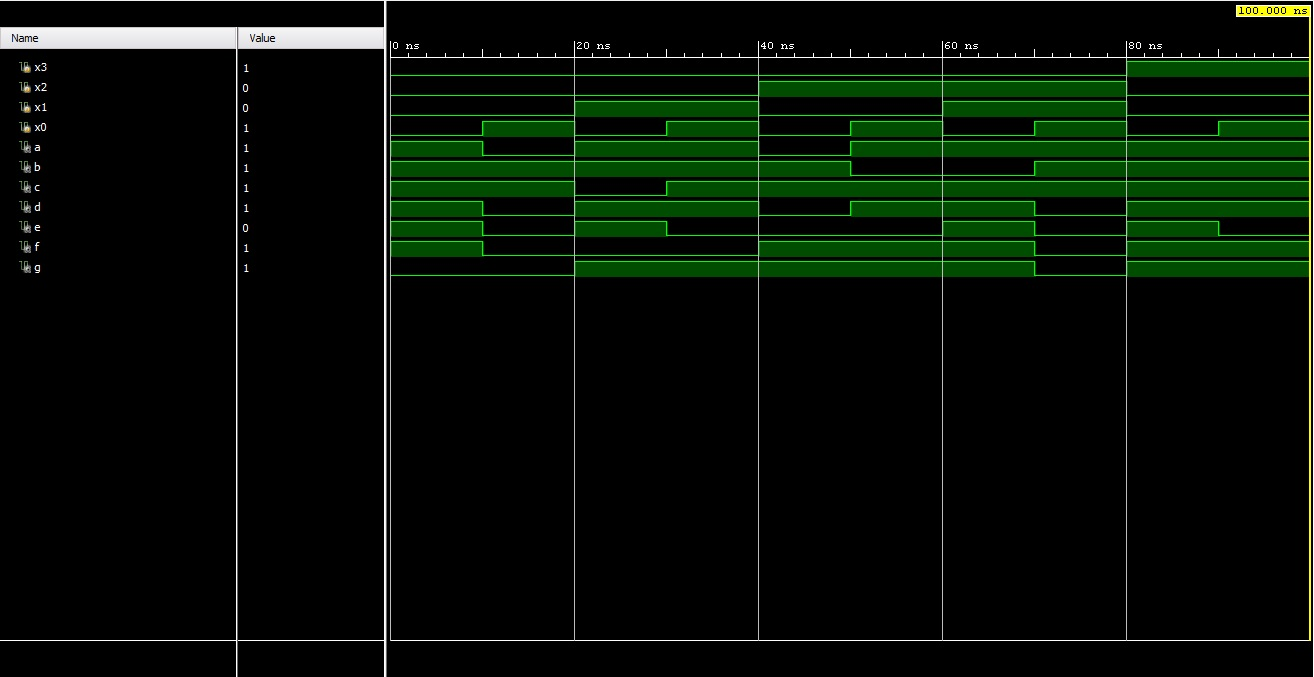
\includegraphics[scale=0.4]{Timing_Diagram}
\caption{The full screen result of the simulation}
\end{figure}

Figure 2 and Figure 3 show zoomed-in screenshots of that in Figure 1.\\

\begin{figure}[h!]
\centering
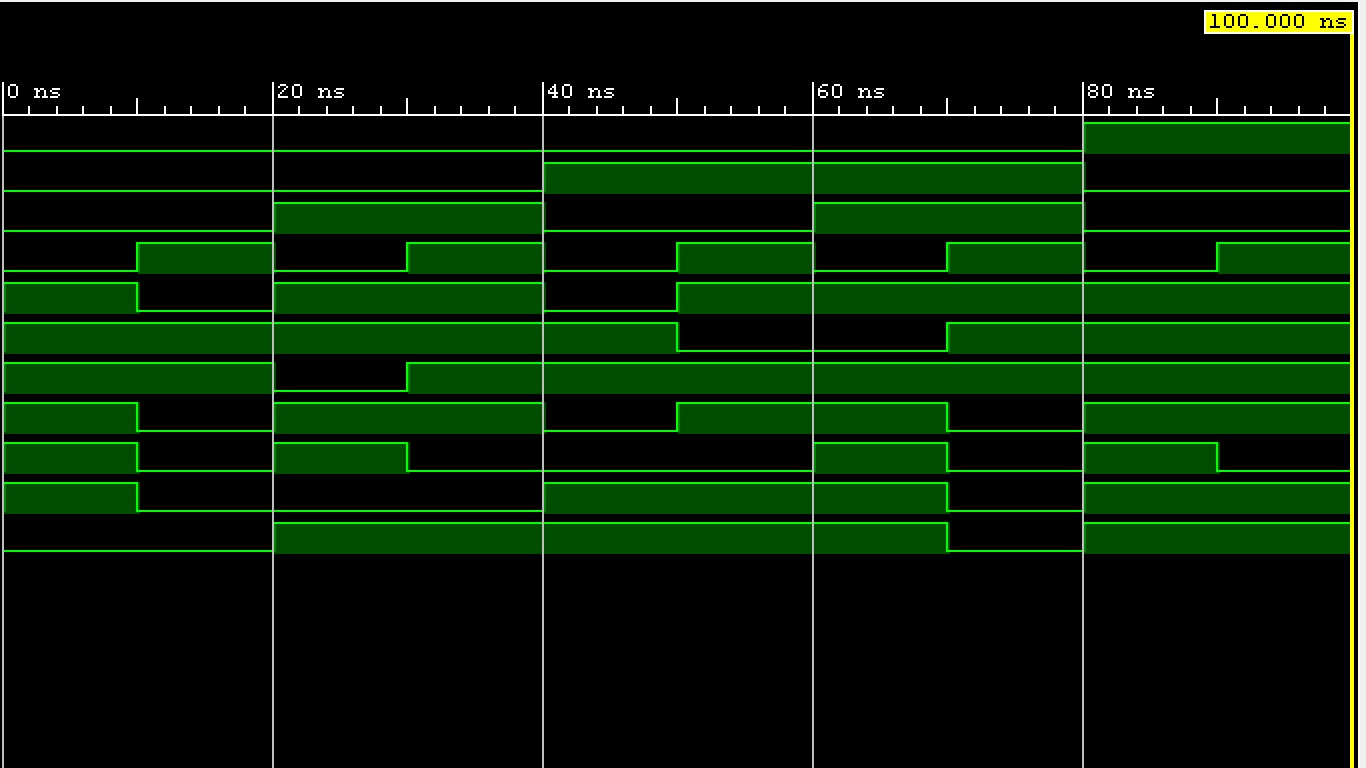
\includegraphics[scale=0.4]{Timing_Diagram-Magnified_Voltages}
\caption{The zoomed-in version of the timing diagram}
\end{figure}

\clearpage

\begin{figure}[h!]
\centering
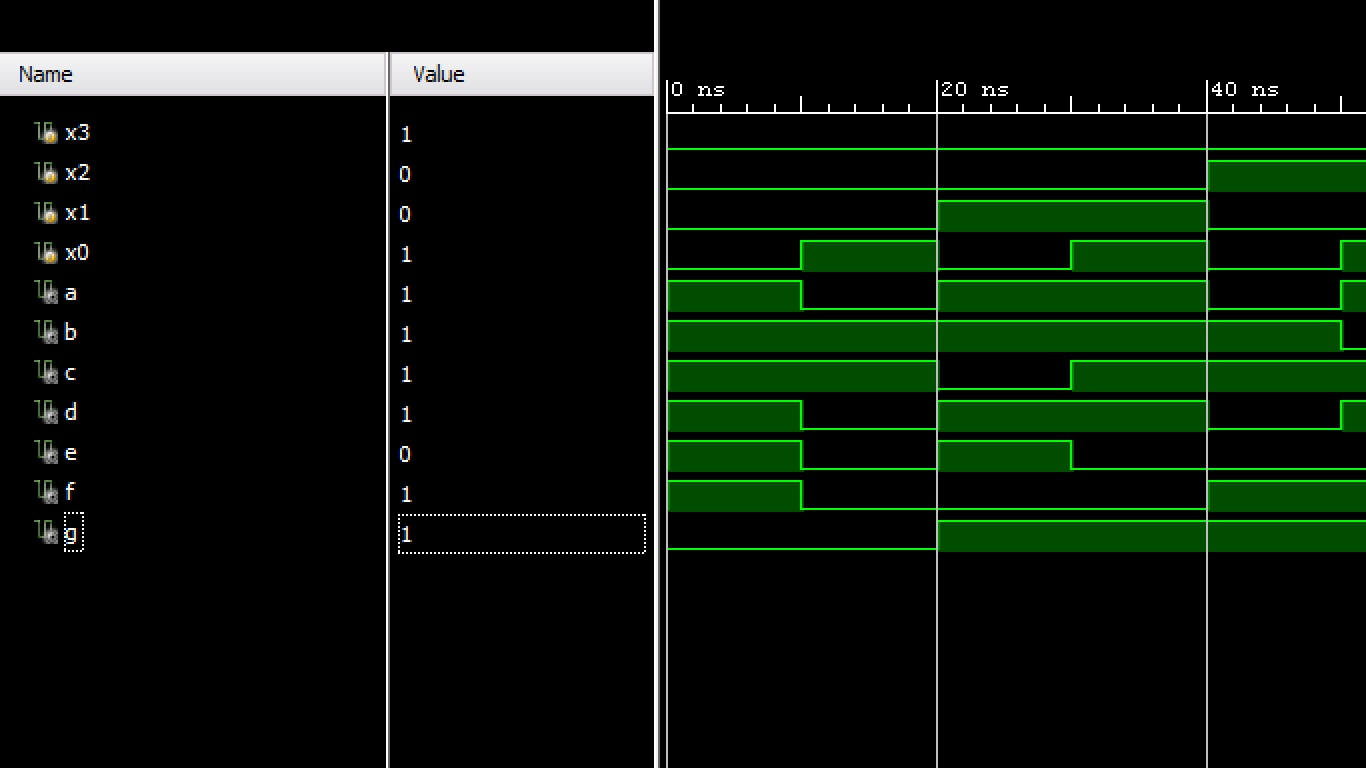
\includegraphics[scale=0.4]{Timing_Diagram-Magnified_IO}
\caption{Another zoomed-in version of the timing diagram}
\end{figure}

To make sense of the result, we must first understand what the green lines 
signify.\\
\\
The left-hand side of the timing diagram shows all of the input and output 
variables. Figure 1 and Figure 3 specifically shows the values of each variable 
precisely when \textbf{x} is given the value of 9. \\
\\
The top four green lines represent the four input variables, while the 
remaining seven represent the output variables. A green line on the bottom 
indicates a logic value of 0, while a green line higher up indicates a logic 
value of 1.  Based on that interpretation, we were able to see that the output 
values are correct for each input combination.\\
\\
The following test bench code was used to generate that simulation result.

\begin{verbatim}
`timescale 1ns / 1ps
//////////////////////////////////////////////////////////////////////////////
// Company: UCLA Henry Samueli School of Engineering and Applied Science
// Engineers: Victor Lai and Dennis Gahm
// Student IDs: 404274720 and 704016107
// 
// Create Date: 05/08/2015 01:05:18 PM
// Design Name: 
// Module Name: csm51a_proj2_tb
// Project Name: Verilog Lab #2
// Target Devices: 
// Tool Versions: 
// Description: 
// 
// Dependencies: 
// 
// Revision:
// Revision 0.01 - File Created
// Additional Comments:
// 
//////////////////////////////////////////////////////////////////////////////

module Top;
reg x3, x2, x1, x0;
wire a, b, c, d, e, f, g;

display_decoder test(x3, x2, x1, x0, a, b, c, d, e, f, g);

initial begin
    
    { x3, x2, x1, x0 } = 0;
    #10
    { x3, x2, x1, x0 } = 1;
    #10
    { x3, x2, x1, x0 } = 2;
    #10
    { x3, x2, x1, x0 } = 3;
    #10
    { x3, x2, x1, x0 } = 4;
    #10
    { x3, x2, x1, x0 } = 5;
    #10
    { x3, x2, x1, x0 } = 6;
    #10
    { x3, x2, x1, x0 } = 7;
    #10
    { x3, x2, x1, x0 } = 8;
    #10
    { x3, x2, x1, x0 } = 9;
    #10
        
    $finish;
end
endmodule

\end{verbatim}

To observe the output values of each input combination, we changed the input 
every 10 nanoseconds.

%----------------------------------------------------------------------------
%	DESIGN REVIEW
%----------------------------------------------------------------------------

\section{Design Review}
Throughout the process of completing this project, we learned many things 
ranging from applying concepts we learned in class to using new software.\\
\\
In this project, we learned how to apply the concepts we learned in class to a 
real-world application. We learned that the mechanism of displaying digits on 
an LED basically just comes from the idea that switching on and off takes
logic values.  \\
\\
There were many points in time when we found the specfication to be ambiguous. 
For example, we did not know whether or not we can have complemented inputs
in our design, so we first assumed that we could use those considering that we 
were almost always able to use those in class. However, when we finally got 
the opportunity to ask the instructor about it, we unfortunately learned that 
complemented inputs are not allowed specifically in the design of a real 
circuit. Consequently, we had to go through the trouble of fixing all of our 
diagrams and drawings to include NOT gates to accommodate those complemented 
inputs.\\
\\
By asking questions, we clarified on many small but yet critical parts of the 
project. It would be helpful if future project specifications are clearer and 
address these issues. The interpretation of a schematic as the one generated 
from Vivado compared to as a circuit representation can cause a team to include
 a schematic that the instructor does not want and ultimately lower their 
score.\\
\\
We also learned a bit about using \LaTeX to generate a professional, 
well-formatted report. We had prior experience using \LaTeX but it was very 
limited, so by doing some research on syntax, we were able to teach ourselves 
things like placing tables and images side by side in a document.\\
\\
The creation of switching expressions using a truth 
table and K-map, the transformation from AND-OR to NAND, and the 
implementation and simulation in Vivado was almost trivial because we 
practiced it often in class. We had to choose between two implementations in 
Vivado - using the behavorial implementation (with the \textit{assign} keyword) 
versus using structural gate primitives . We decided to use the behavorial 
implementation but include as comments the structural approach. \\
\\
We spent a good chunk of our time drawing out the schematics on the computer 
using Paint and playing around with \LaTeX to format the text, images, and 
tables nicely together. Nevertheless, the most important aspects of the 
project were the application of the concepts learned in class to a real world 
problem, learning \LaTeX as it will be helpful for future reports, and 
learning Vivado, which will be useful for future projects involving logic 
gates.

%----------------------------------------------------------------------------
%	TEAM MEMBER CONTRIBUTIONS
%----------------------------------------------------------------------------

\section{Team Member Contributions}
Each team member assumed a relatively equal share of the worload of this 
project.\\
\\
Dennis worked on writing most of the text of the report. He first created the 
design on his own before chiecking his work with Victor. In particular, Dennis 
was keen in pointing out to Victor that single terms in the switching 
expression can be represented as single wires rather than using an AND gate 
to take the same term twice as inputs. He also checked the 
correctness of the simulation.  In addition, he clarified the specification 
about complemented inputs so that the team used NOT gates for the correct 
minimal expression and network. \\
\\
Victor worked on the design, Vivado code and simulation, and the \LaTeX portions
 of the report. He created the schematics (using Paint) for the report and 
put together the professional layout using \LaTeX. He was the first to 
formulate the design on paper on his own.  The pencil-and-paper design in 
Section 6.7 shows his work which was later verified by Dennis. \\
\\
Overall, each member of the team contributed to roughly 50\% to the completion 
of the project.

%----------------------------------------------------------------------------
%	APPENDIX
%----------------------------------------------------------------------------

\section{Appendix}
The following diagrams and screenshots show our complete set of worksheets 
worked out using paper and pencil. They illustrate how we came up with the 
minimal NAND-NAND expressions in Section 1. Let $ \vec{x} = 
\{ x_3, x_2, x_1, x_0 \} $ represent the BCD code.\\


\subsection{Inputs and Outputs}
Professor Yutao He always reminds his students to draw "The Box" when starting 
to design and analyze a digital system. Remembering that piece of advice, we 
started our design by drawing it to get a sense of the inputs and outputs. 
Those inputs and outputs are depicted in Figure 4. \\

\clearpage

\begin{figure}[h!]
\centering
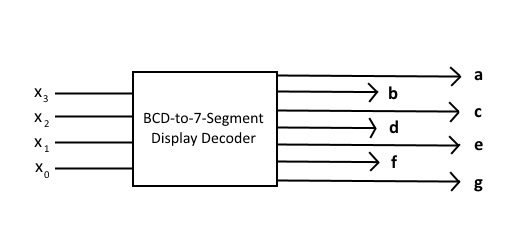
\includegraphics[scale=0.7]{Box}
\caption{"The Box!"}
\end{figure}


\subsection{Encoding Schemes}
As given in the specification, the encoding scheme of the inputs of the 
network system are shown in Table 1, while that of the outputs are shown in 
Table 2.\\

\begin{table} [hp]
\begin{center}

\begin{tabular}{ c | c c c c }
\centering

  Decimal No. & $x_3$ & $x_2$ & $x_1$ & $x_0$ \\
  \hline
  0           & 0     & 0     & 0     & 0     \\
  1           & 0     & 0     & 0     & 1     \\
  2           & 0     & 0     & 1     & 0     \\
  3           & 0     & 0     & 1     & 1     \\
  4           & 0     & 1     & 0     & 0     \\
  5           & 0     & 1     & 0     & 1     \\
  6           & 0     & 1     & 1     & 0     \\
  7           & 0     & 1     & 1     & 1     \\
  8           & 1     & 0     & 0     & 0     \\
  9           & 1     & 0     & 0     & 1     \\

\end{tabular}
\caption{The Input Encoding Scheme}
\end{center}
\label{table:1}
\end{table}

\begin{table} [h!]
\begin{center}
\begin{tabular}{ c | c }
\centering

  Segment State & Binary Code \\
  \hline
  ON            & 1           \\
  OFF           & 0           \\

\end{tabular}
\caption{The Output Encoding Scheme}
\end{center}
\label{table:2}
\end{table}


\subsection{Truth Table}
Based on the encoding schemes of the input and output, the truth table is 
shown in Table 3.\\

\begin{table} [h!]
\begin{center}
\begin{tabular}{ c c c c | c c c c c c c }
\centering

  $x_3$ & $x_2$ & $x_1$ & $x_0$ & a & b & c & d & e & f & g \\
  \hline
  0     & 0     & 0     & 0     & 1 & 1 & 1 & 1 & 1 & 1 & 0 \\
  0     & 0     & 0     & 1     & 0 & 1 & 1 & 0 & 0 & 0 & 0 \\
  0     & 0     & 1     & 0     & 1 & 1 & 0 & 1 & 1 & 0 & 1 \\
  0     & 0     & 1     & 1     & 1 & 1 & 1 & 1 & 0 & 0 & 1 \\
  0     & 1     & 0     & 0     & 0 & 1 & 1 & 0 & 0 & 1 & 1 \\
  0     & 1     & 0     & 1     & 1 & 0 & 1 & 1 & 0 & 1 & 1 \\
  0     & 1     & 1     & 0     & 1 & 0 & 1 & 1 & 1 & 1 & 1 \\
  0     & 1     & 1     & 1     & 1 & 1 & 1 & 0 & 0 & 0 & 0 \\
  1     & 0     & 0     & 0     & 1 & 1 & 1 & 1 & 1 & 1 & 1 \\
  1     & 0     & 0     & 1     & 1 & 1 & 1 & 1 & 0 & 1 & 1 \\
  1     & 0     & 1     & 0     & - & - & - & - & - & - & - \\
  1     & 0     & 1     & 1     & - & - & - & - & - & - & - \\
  1     & 1     & 0     & 0     & - & - & - & - & - & - & - \\
  1     & 1     & 0     & 1     & - & - & - & - & - & - & - \\
  1     & 1     & 1     & 0     & - & - & - & - & - & - & - \\
  1     & 1     & 1     & 1     & - & - & - & - & - & - & - \\

\end{tabular}
\caption{Truth Table}
\end{center}
\label{table:3}
\end{table}


\subsection{Minimization Procedure}
We used K-maps in order to first find the minimal sum of products for each 
output. The red circles in the K-maps shown below indicate the prime 
implicants (including the essential ones).\\
%\pagebreak

\begin{table}[h!]
\begin{tabular}{ c c }
\centering
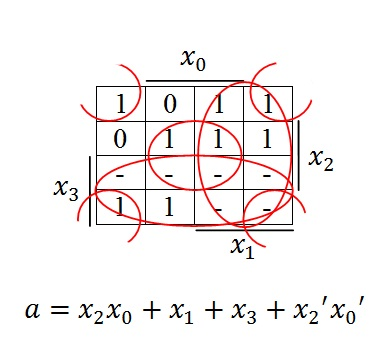
\includegraphics[scale=0.6]{a-KMap} &
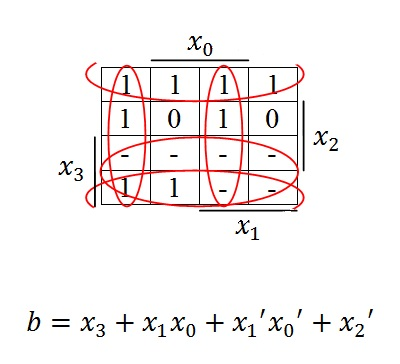
\includegraphics[scale=0.6]{b-KMap} \\
\end{tabular}
\end{table}

\pagebreak

\begin{table}[h!]
\begin{tabular}{ c c }
\centering
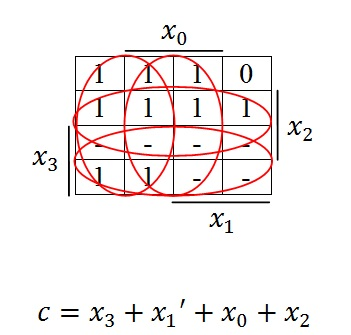
\includegraphics[scale=0.6]{c-KMap} &
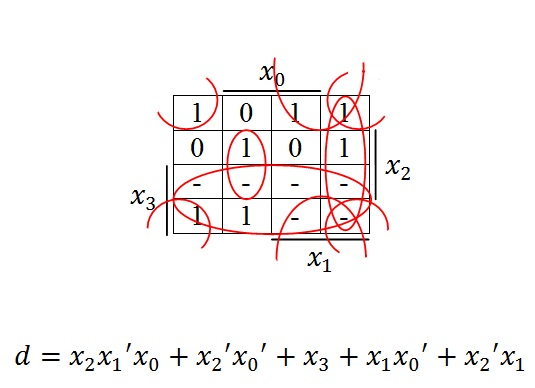
\includegraphics[scale=0.6]{d-KMap} \\
\end{tabular}
\end{table}

\begin{table}[h!]
\begin{tabular}{ c c }
\centering
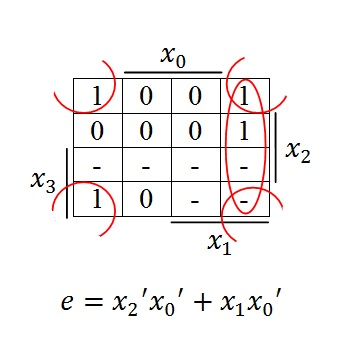
\includegraphics[scale=0.6]{e-KMap} &
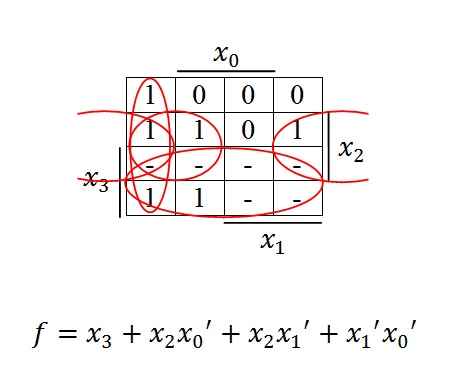
\includegraphics[scale=0.6]{f-KMap} \\
\end{tabular}
\end{table}

\begin{figure*}[h!]
\centering
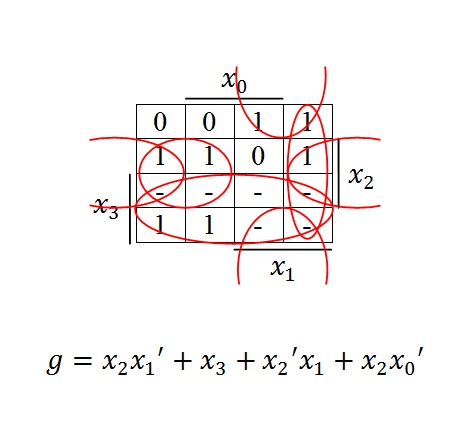
\includegraphics[scale=0.6]{g-KMap}
%\caption{K-map for \textit{g}}
\end{figure*}

\pagebreak

From our work, we found that every minimal sum of products is unique except 
that of \textit{g}.


\subsection{Transformation Procedure}
To transform our AND-OR functions into NAND-NAND functions, we used bubble 
logic. The following diagrams depict the transformation.

\begin{figure*}[hp]
\centering
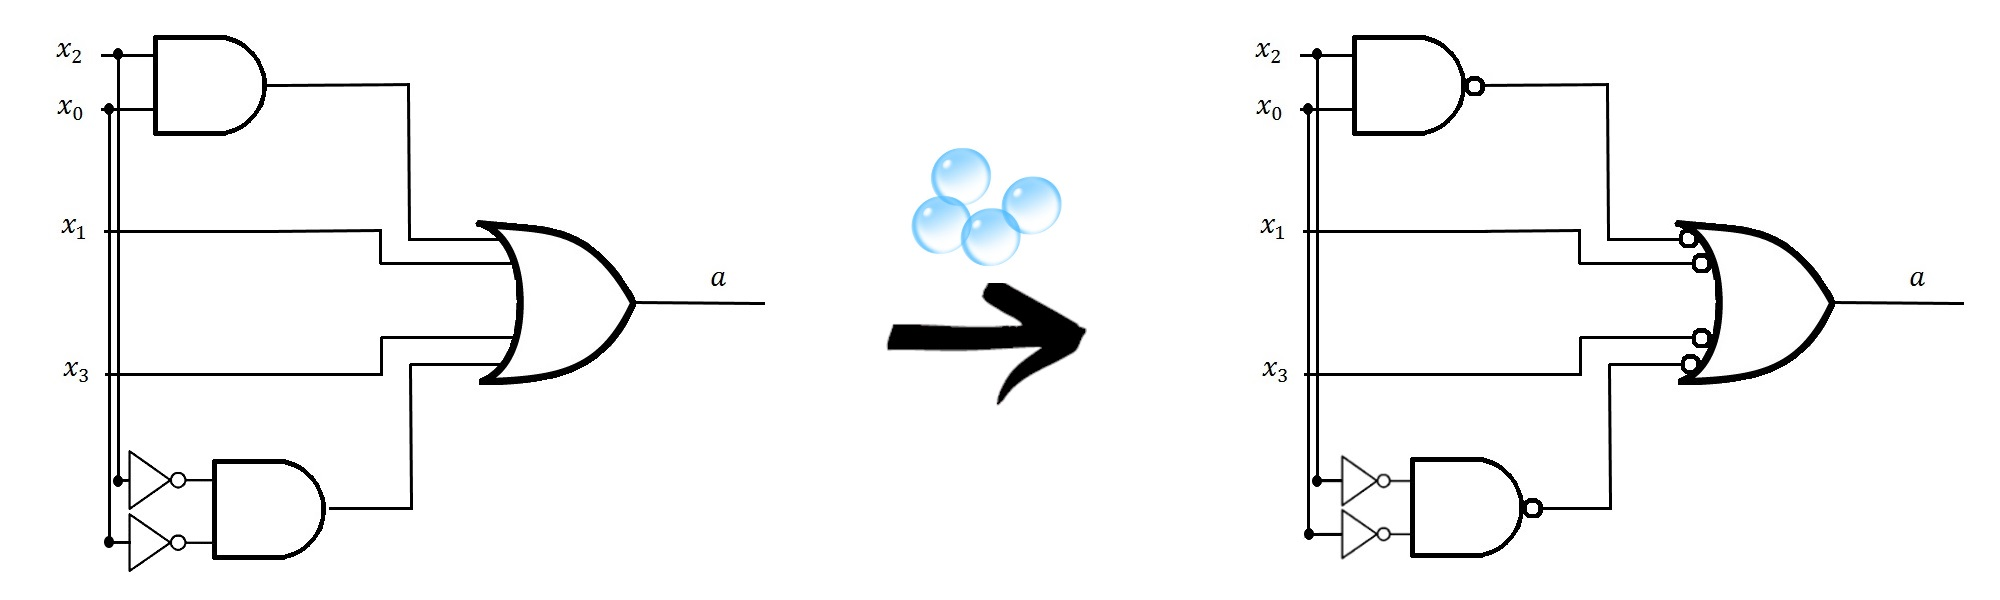
\includegraphics[scale=0.25]{a-transformation}
\end{figure*}

\begin{figure*}[hp]
\centering
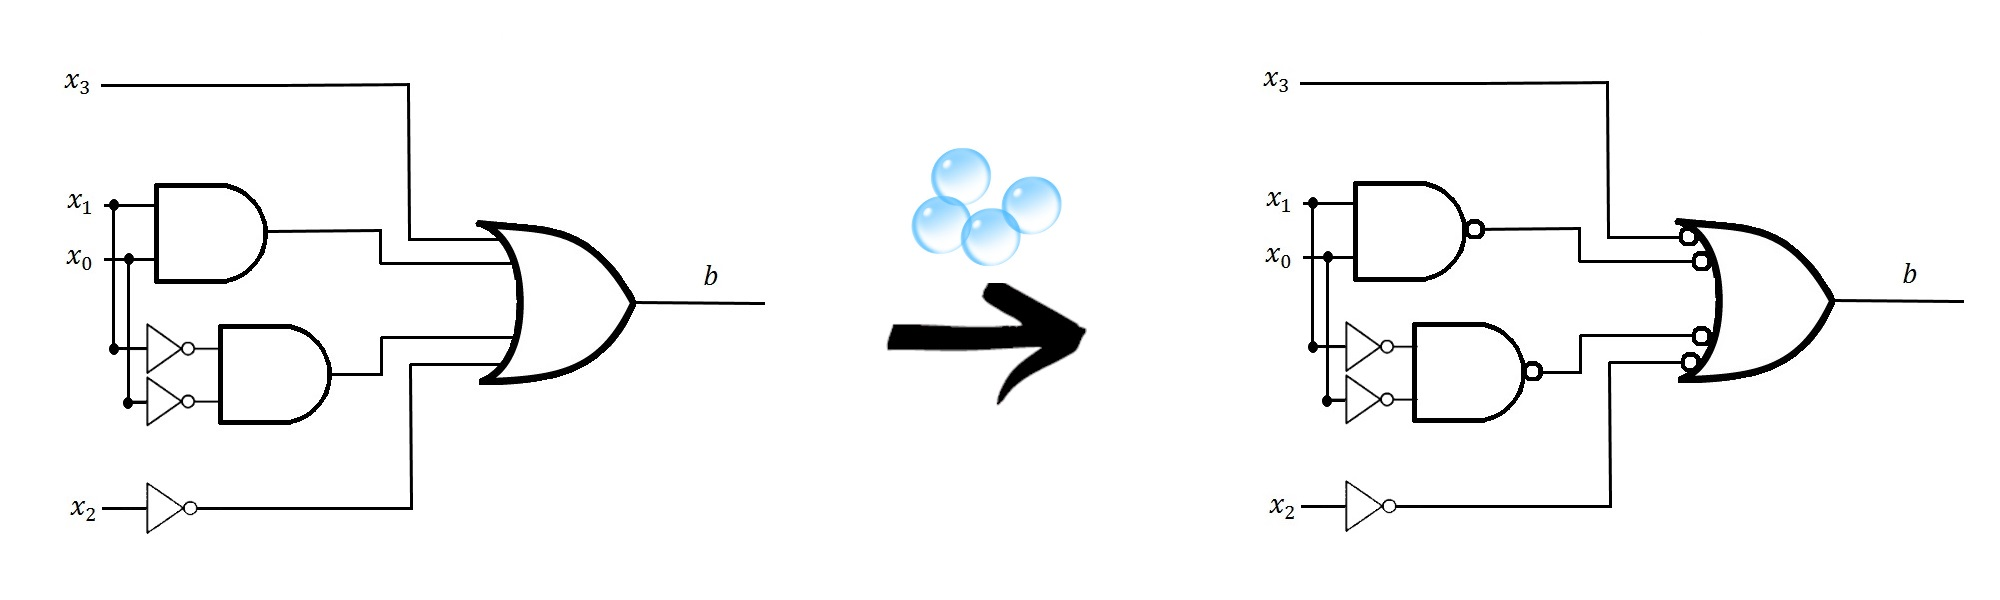
\includegraphics[scale=0.25]{b-transformation}
\end{figure*}

\begin{figure*}[hp]
\centering
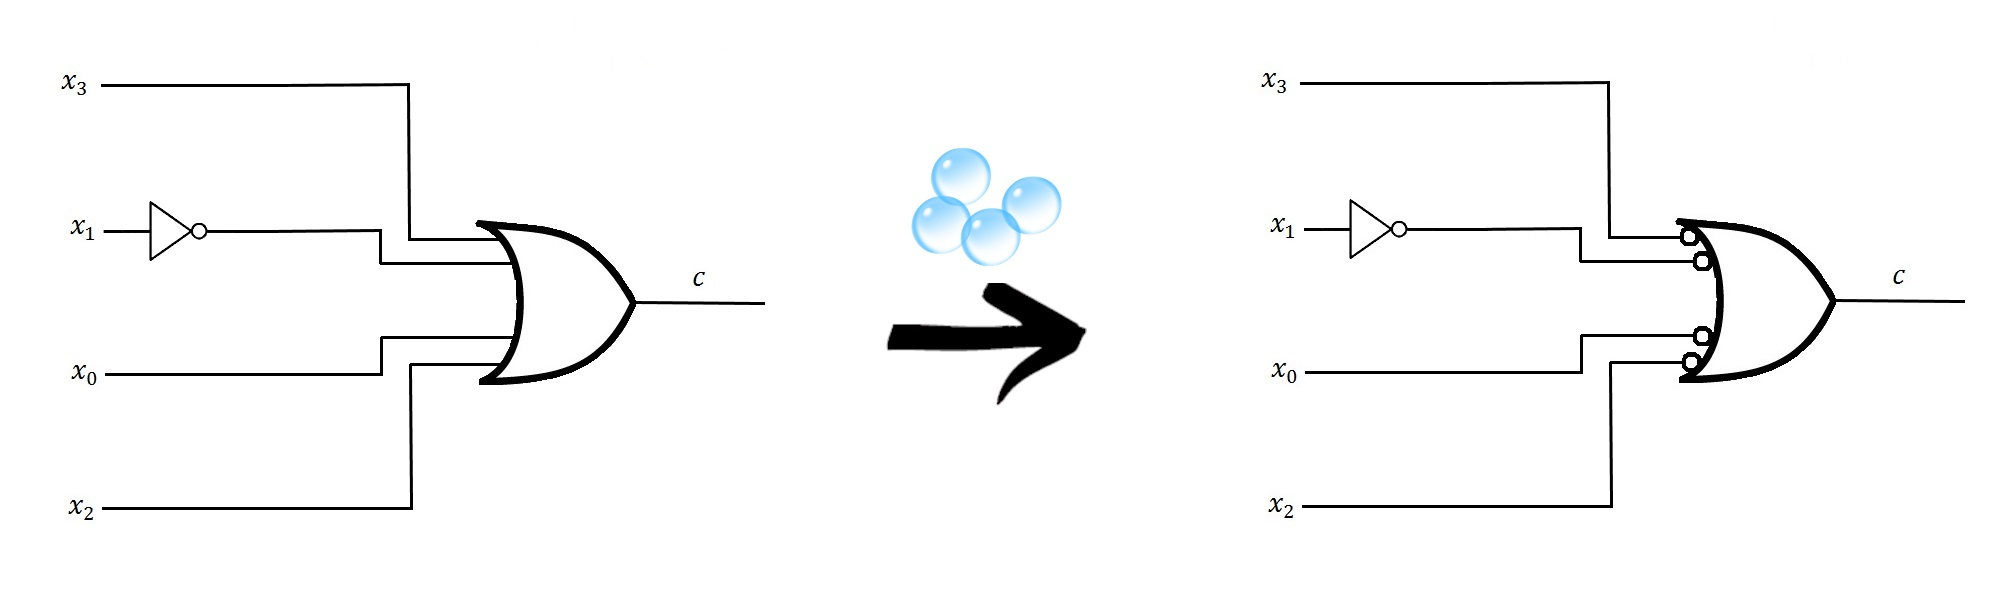
\includegraphics[scale=0.25]{c-transformation}
\end{figure*}

\begin{figure*}[hp]
\centering
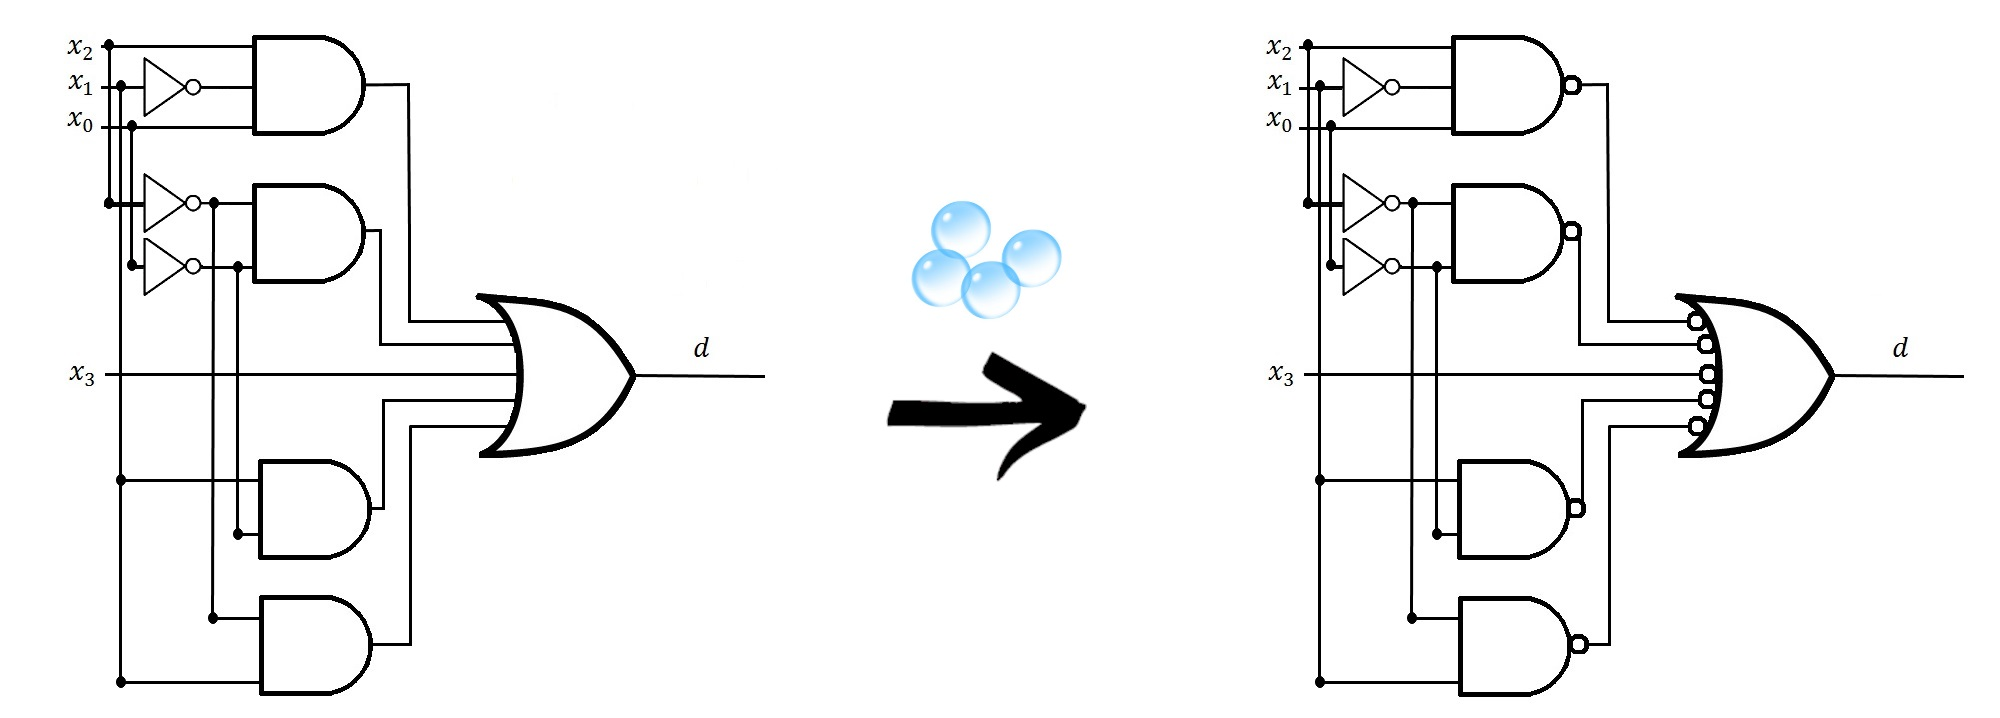
\includegraphics[scale=0.25]{d-transformation}
\end{figure*}

\begin{figure*}[hp]
\centering
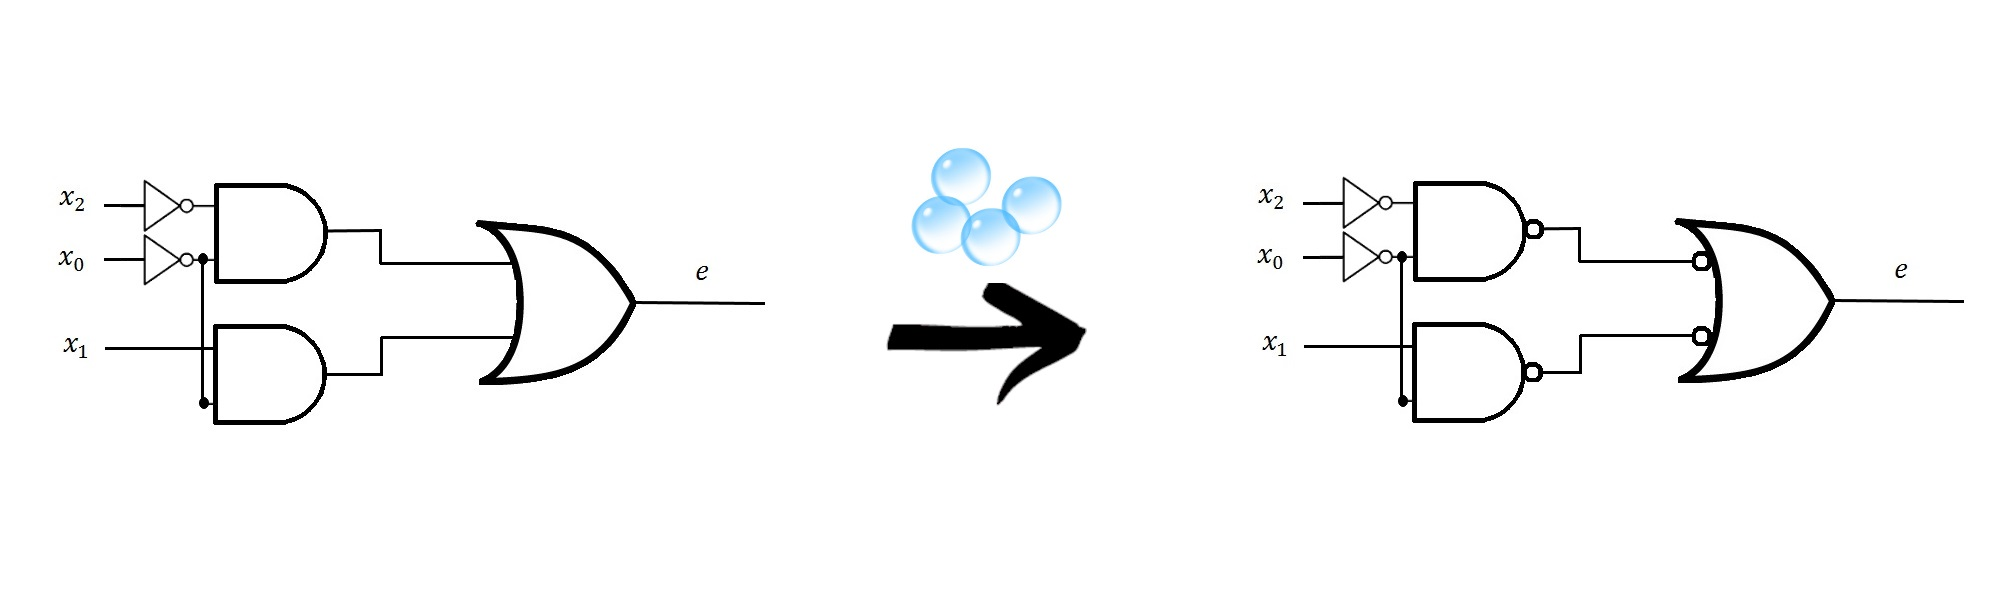
\includegraphics[scale=0.25]{e-transformation}
\end{figure*}

\begin{figure*}[hp]
\centering
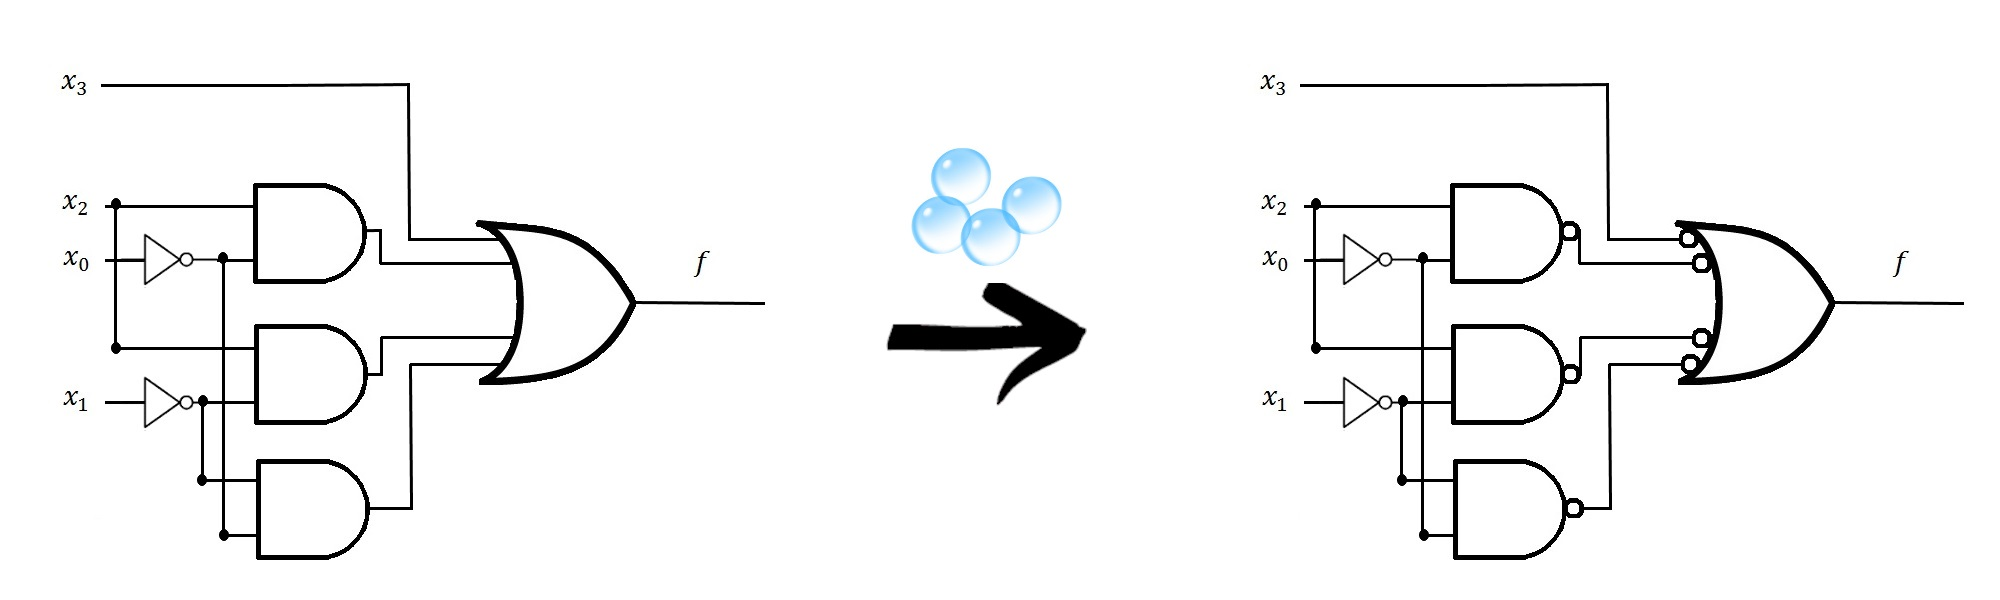
\includegraphics[scale=0.25]{f-transformation}
\end{figure*}

\begin{figure*}[hp]
\centering
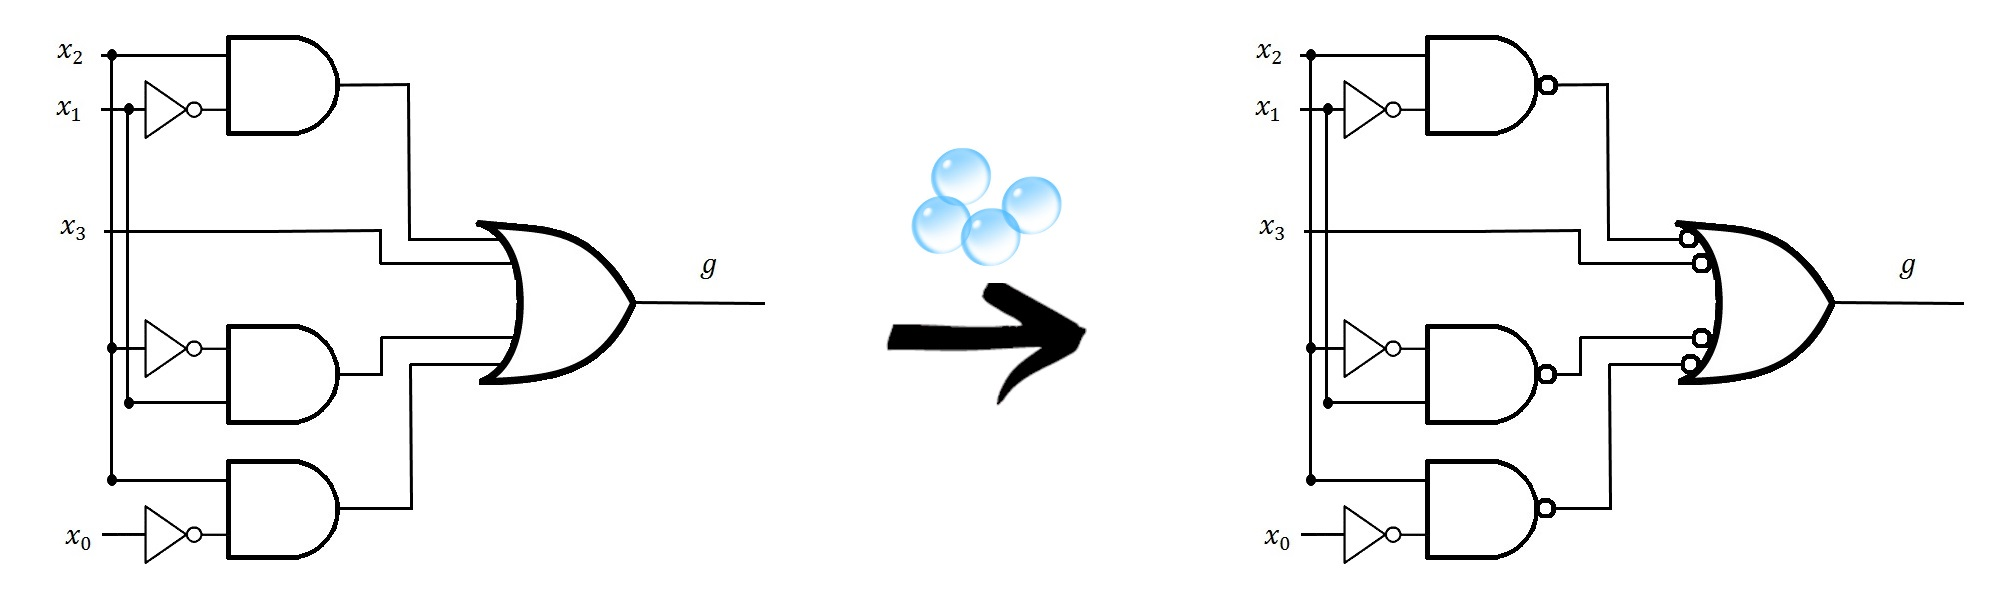
\includegraphics[scale=0.25]{g-transformation}
\end{figure*}

\clearpage


\subsection{Final Minimal Expressions}
After transforming the AND-OR functions using bubble logic, we converted the OR
gate with negated inputs into a NAND gate (for each function).  Moreover, we 
negated the inputs with single wires. Likewise, we used De Morgan's Law to 
ultimately get the equivalent minimal NAND-NAND expressions. As a result, we 
obtained the following networks and their corresponding expressions.\\

\begin{table}[h!]
\begin{tabular}{ c c }
\centering
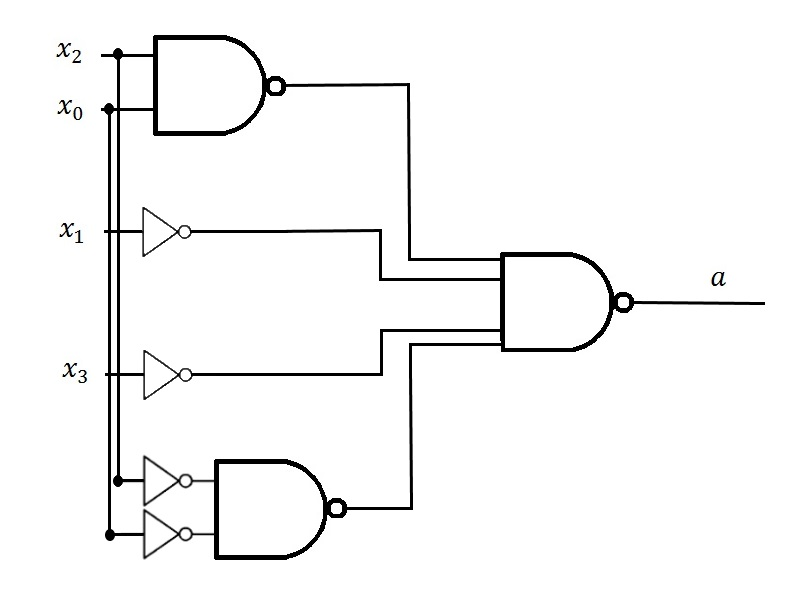
\includegraphics[scale=0.25]{a-NAND-NAND} &
\includegraphics[scale=0.25]{b-NAND-NAND} \\
$a = [ (x_2 x_0)'  (x_1)'  (x_3)'  (x'_2 x'_0)' ]'$ &
$b = [ (x_3)' (x_1 x_0)' (x'_1 x'_0)' x_2 ]'$ \\
\end{tabular}
\end{table}

\begin{table}[h!]
\begin{tabular}{ c c }
\centering
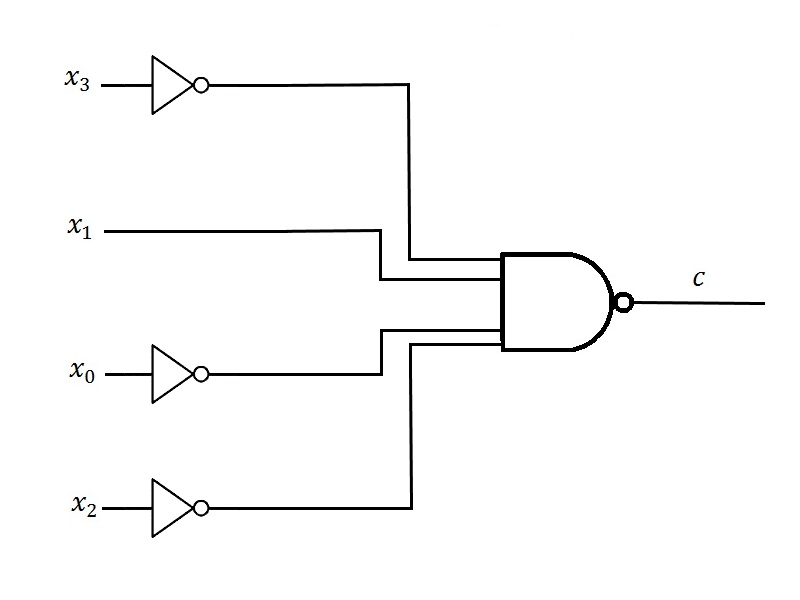
\includegraphics[scale=0.25]{c-NAND-NAND} &
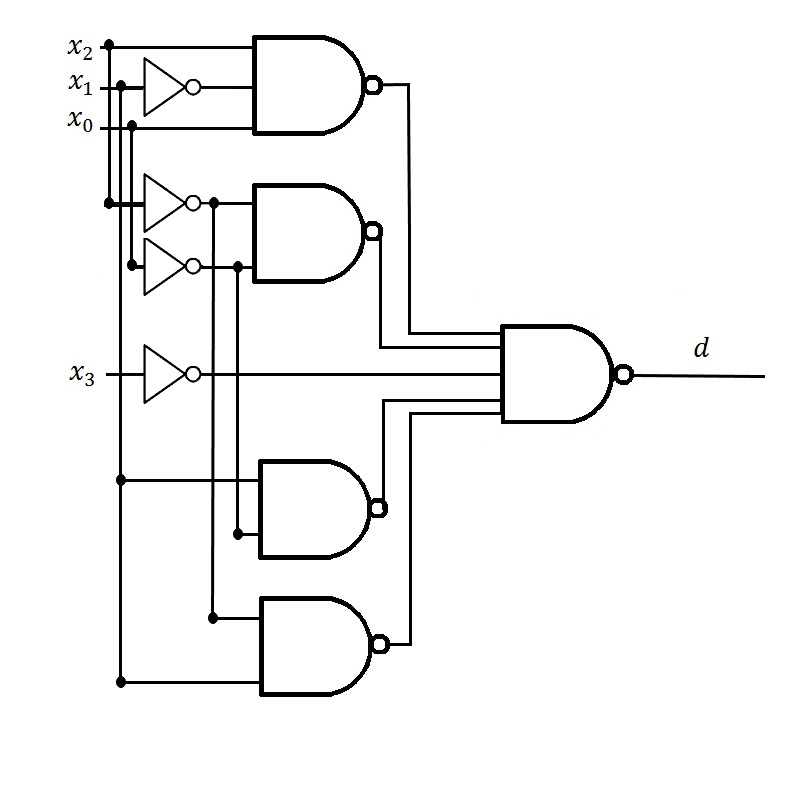
\includegraphics[scale=0.25]{d-NAND-NAND} \\
$c = [ (x_3)' x_1 (x_0)' (x_2)' ]'$ &
$d = [ (x_2 x'_1 x_0)' (x'_2 x'_0)' (x_3)' (x_1 x'_0)' (x'_2 x_1)' ]'$ \\
\end{tabular}
\end{table}

\clearpage

\begin{table}[h!]
\begin{tabular}{ c c }
\centering
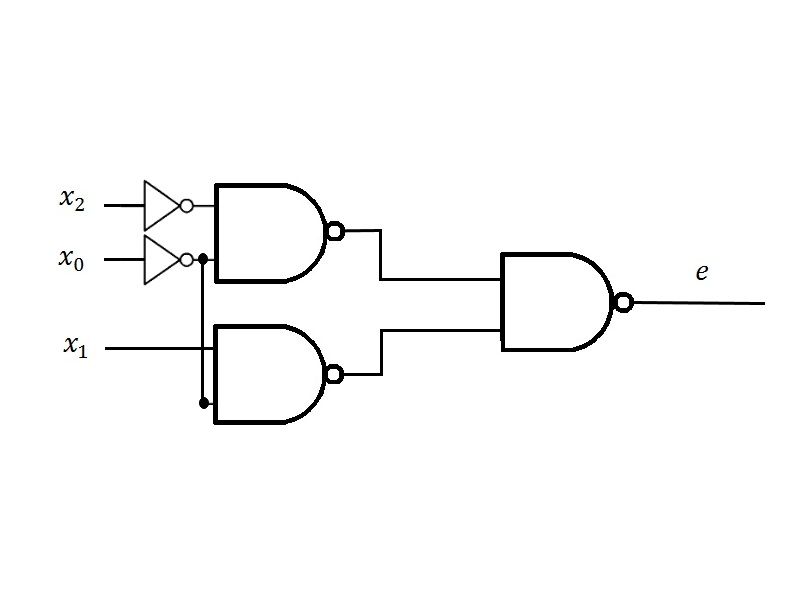
\includegraphics[scale=0.25]{e-NAND-NAND} &
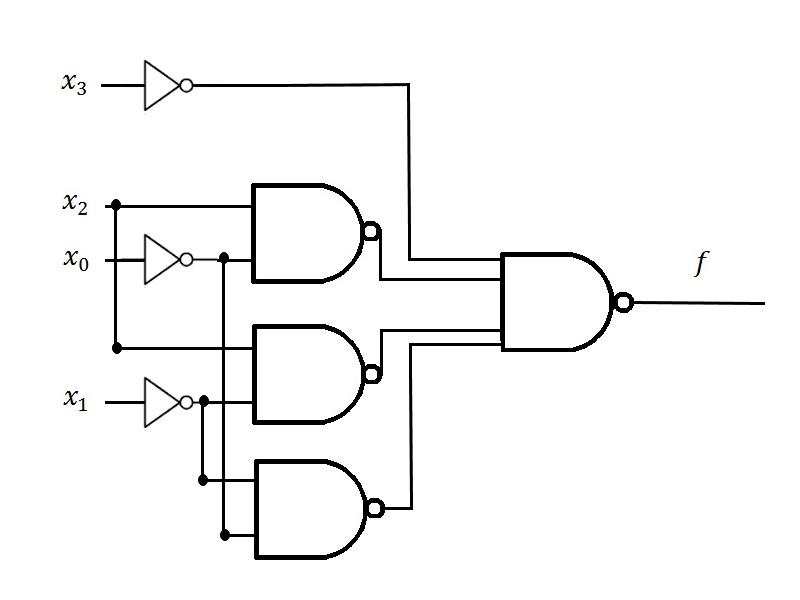
\includegraphics[scale=0.25]{f-NAND-NAND} \\
$e = [ (x'_2 x'_0)' (x_1 x'_0)' ]'$ &
$f = [ (x_3)' (x_2 x'_0)' (x_2 x'_1)' (x'_1 x'_0)' ]'$ \\
\end{tabular}
\end{table}

\begin{figure*}[h!]
\centering
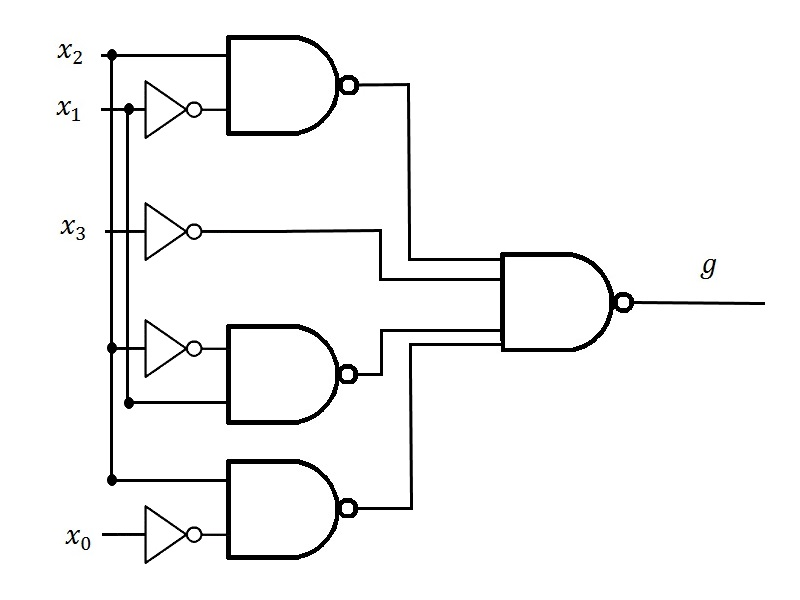
\includegraphics[scale=0.25]{g-NAND-NAND}
%\caption{$g = [ (x_2 x'_1)' (x_3)' (x'_2 x_1)' (x_2 x'_0)' ]'$}
\end{figure*}
\begin{equation*}
\begin{split}
g & = [ (x_2 x'_1)' (x_3)' (x'_2 x_1)' (x_2 x'_0)' ]' \\
\end{split}
\end{equation*}

\clearpage

\subsection{Paper-and-Pencil Design}
The following screenshots show our preliminary work done using paper and 
pencil.\\
\begin{figure}[h!]
\centering
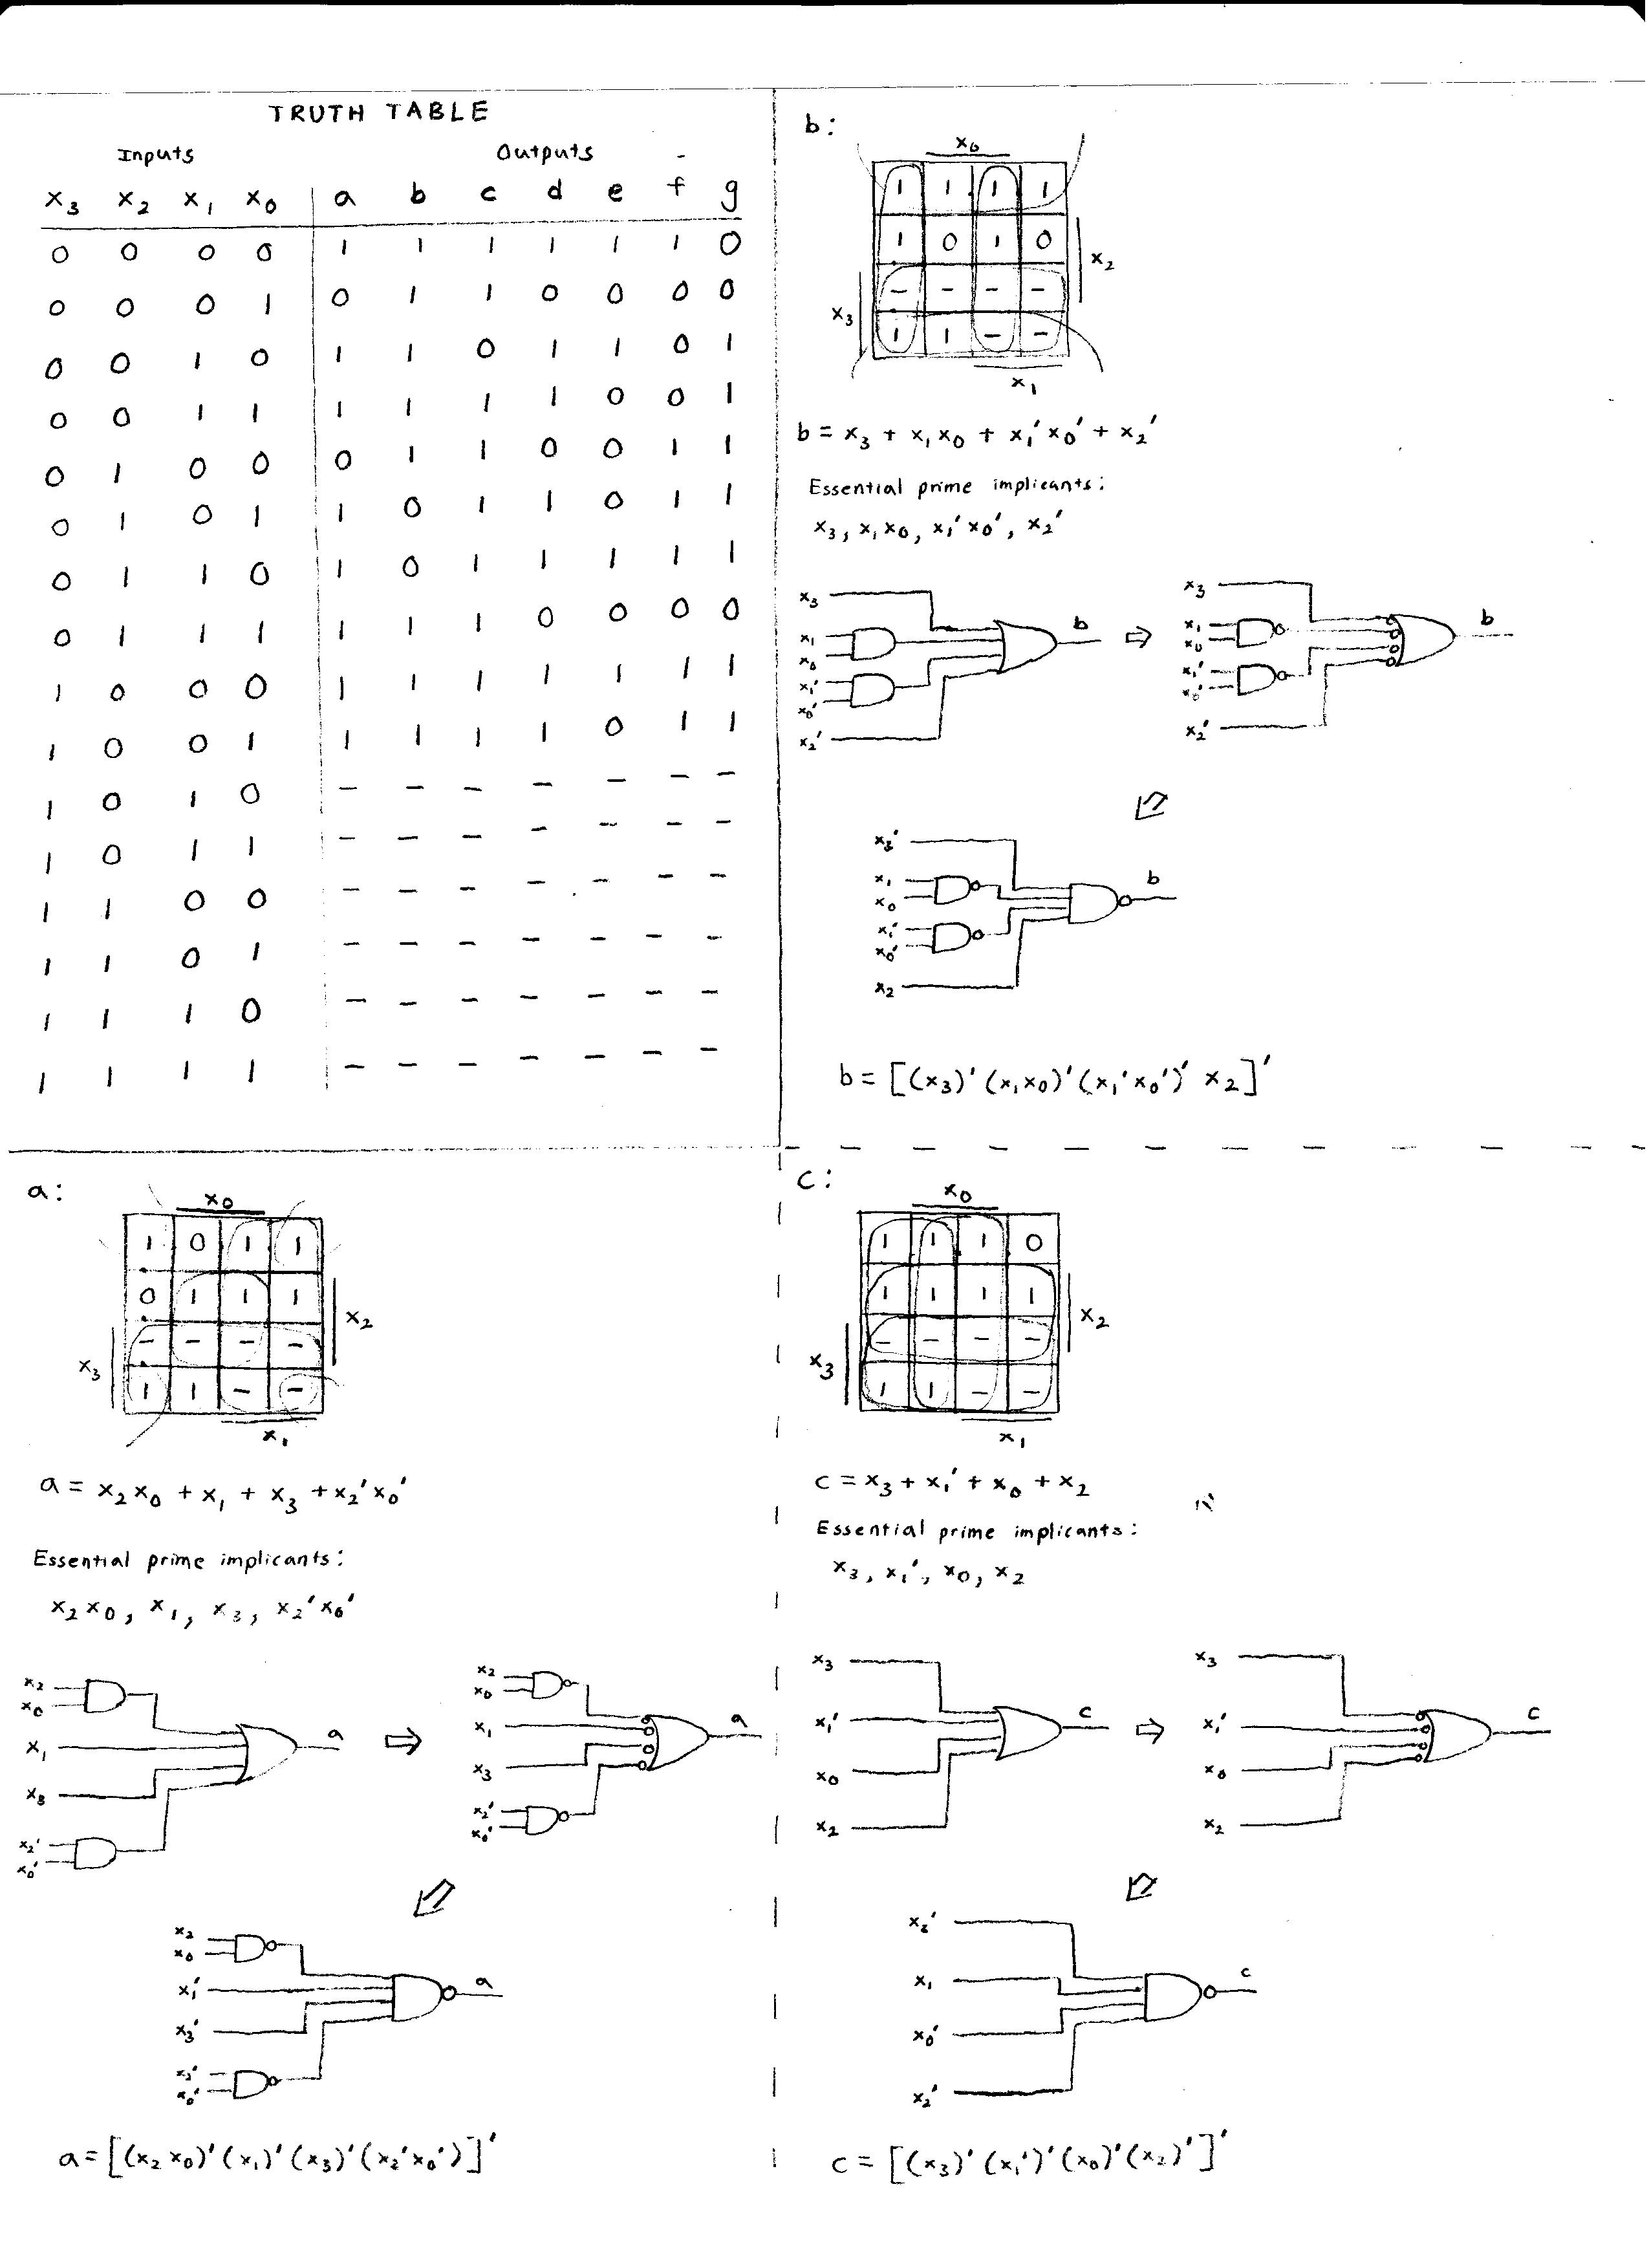
\includegraphics[scale=0.5]{Worksheet(1)}
\caption{First page of our work}
\end{figure}

\begin{figure}[h!]
\centering
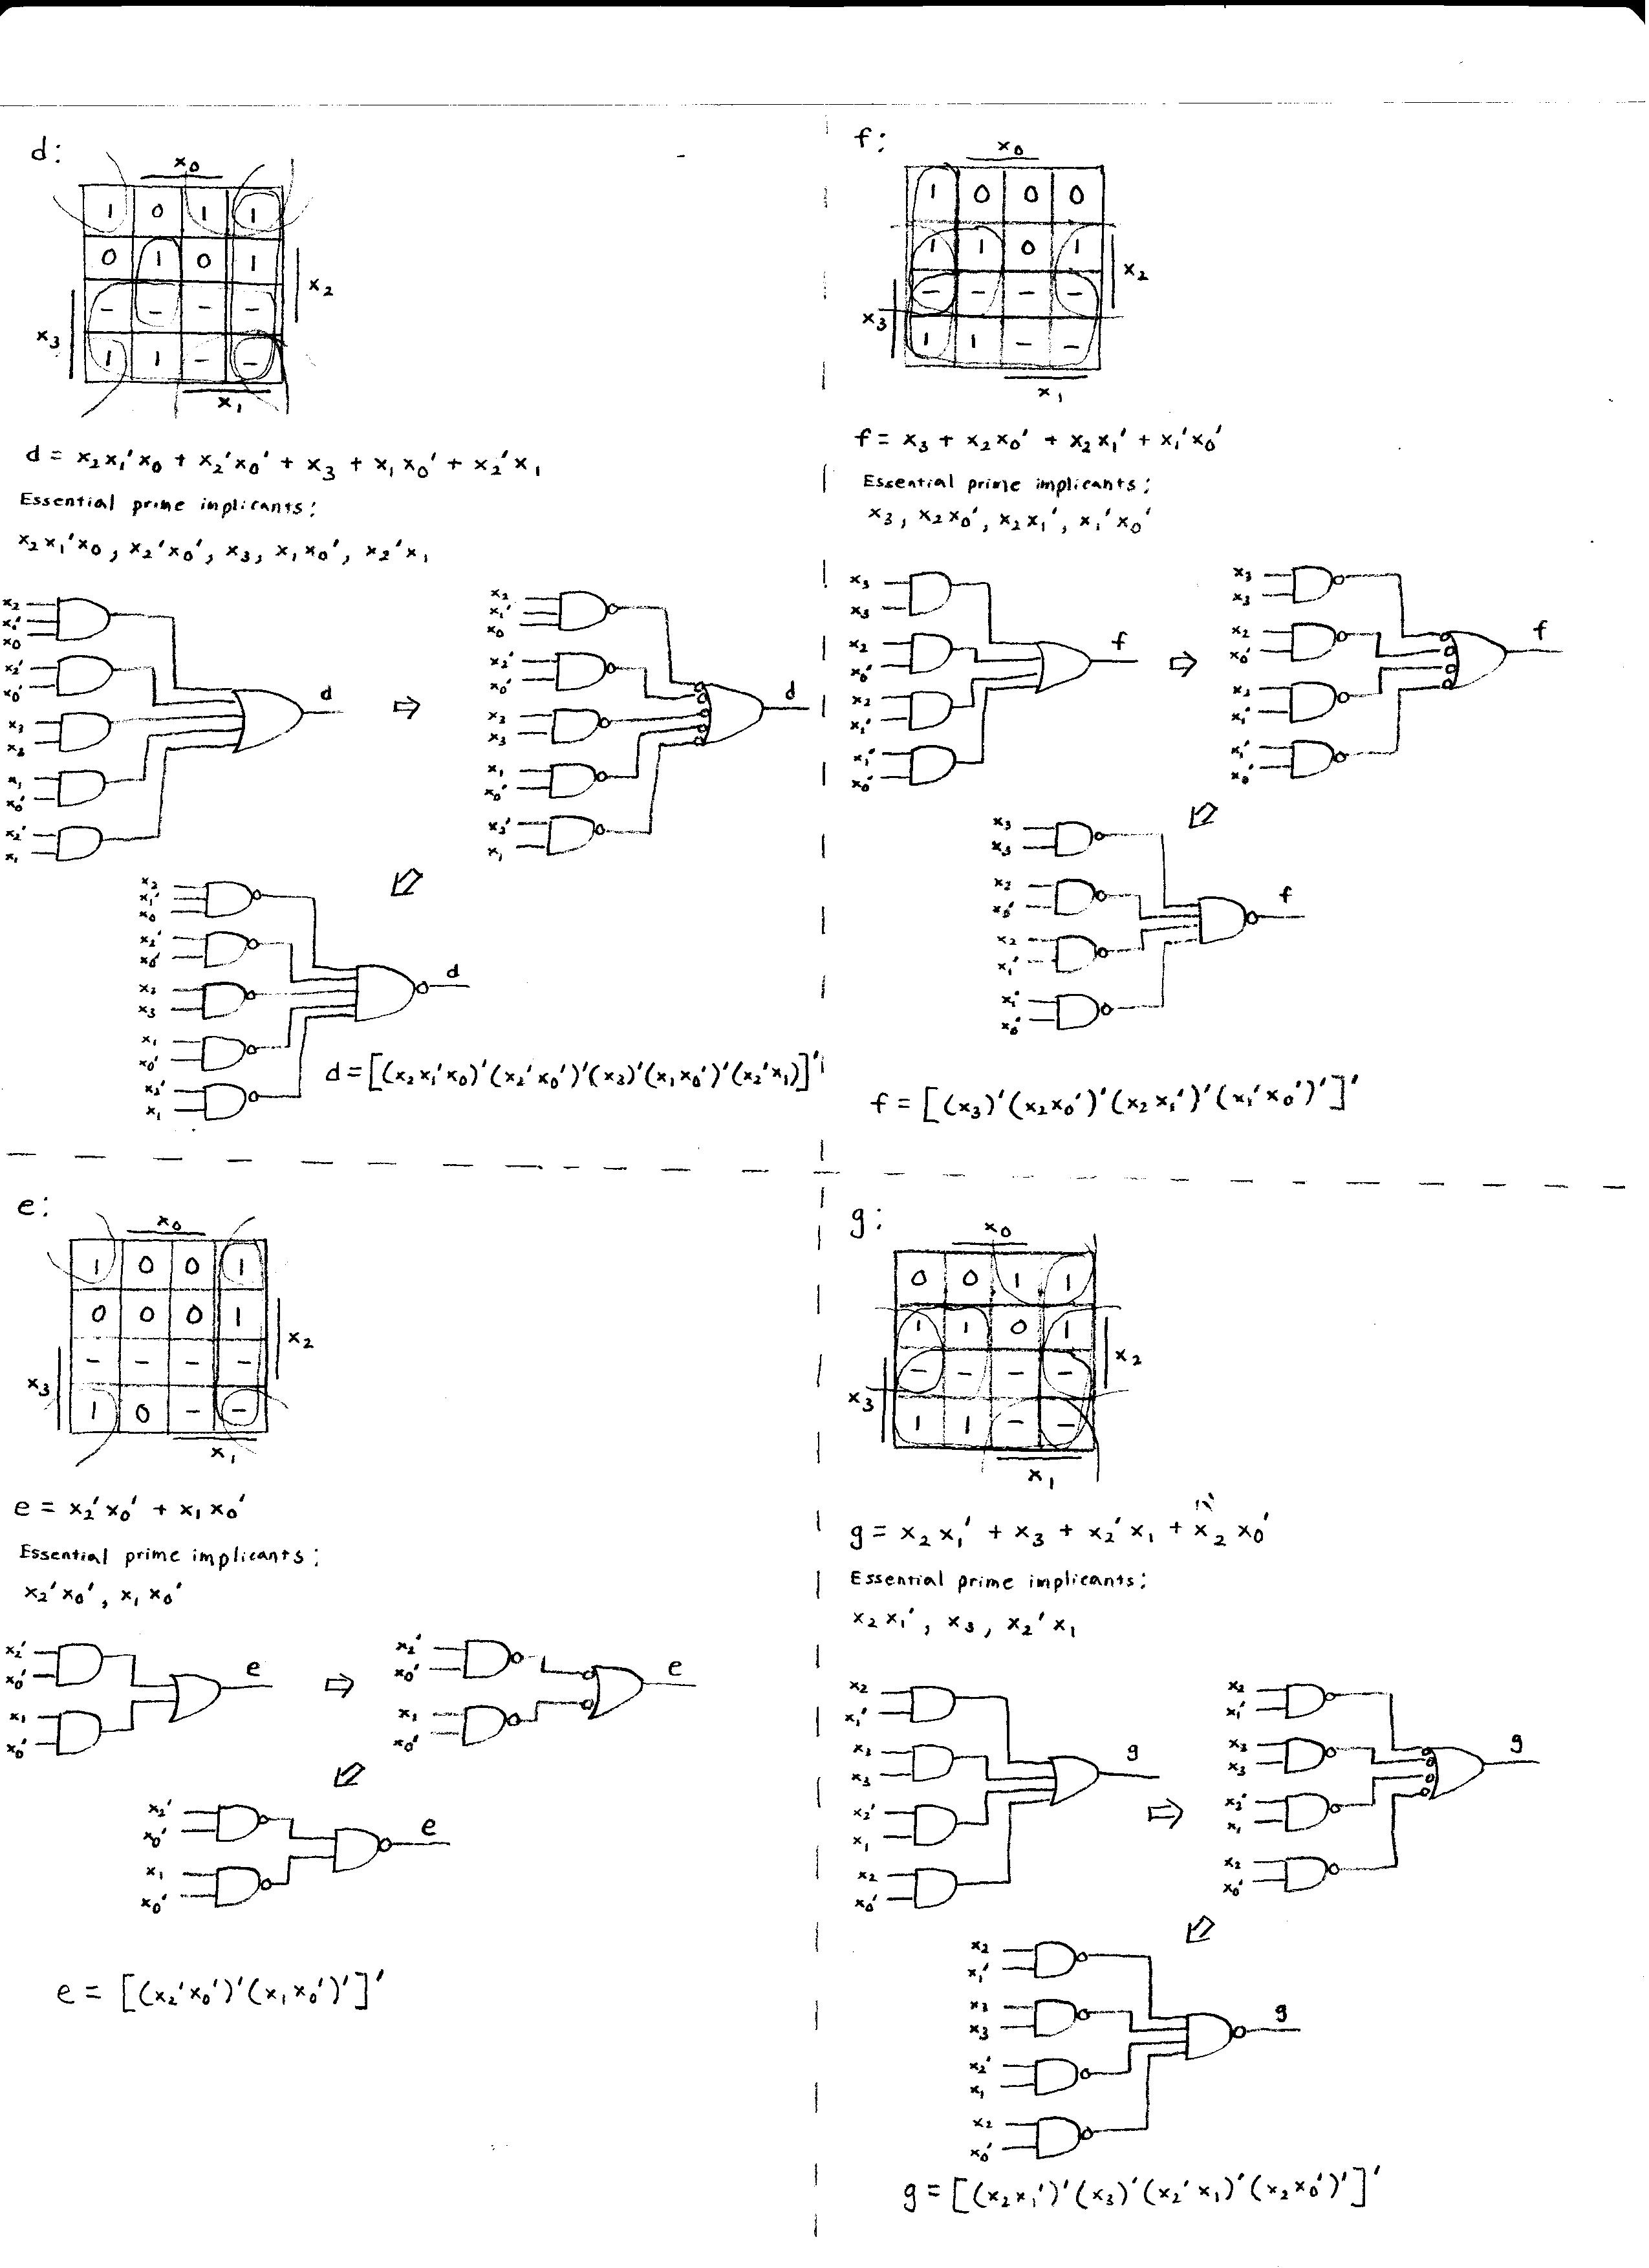
\includegraphics[scale=0.5]{Worksheet(2)}
\caption{Second page of our work}
\end{figure}

%----------------------------------------------------------------------------
\end{document}